% !TeX spellcheck = en_US

\chapter{Results}

\section{\ref{PS:Q:Feasibility}: Does our prototype work?}
Presented below in \cref{fig:graphicalInterface} is shown a screenshot of the graphical interface while the decentralized solution is running 5 turbines. The global setpoint for power production is at 2000, illustrated by the red line and global power production is illustrated by the black line. The blue line illustrates the maximum available power production for the wind farm while the lines in the bottom around 400 is the power production of each individual turbine.

\begin{figure} [!h]
	\centering
	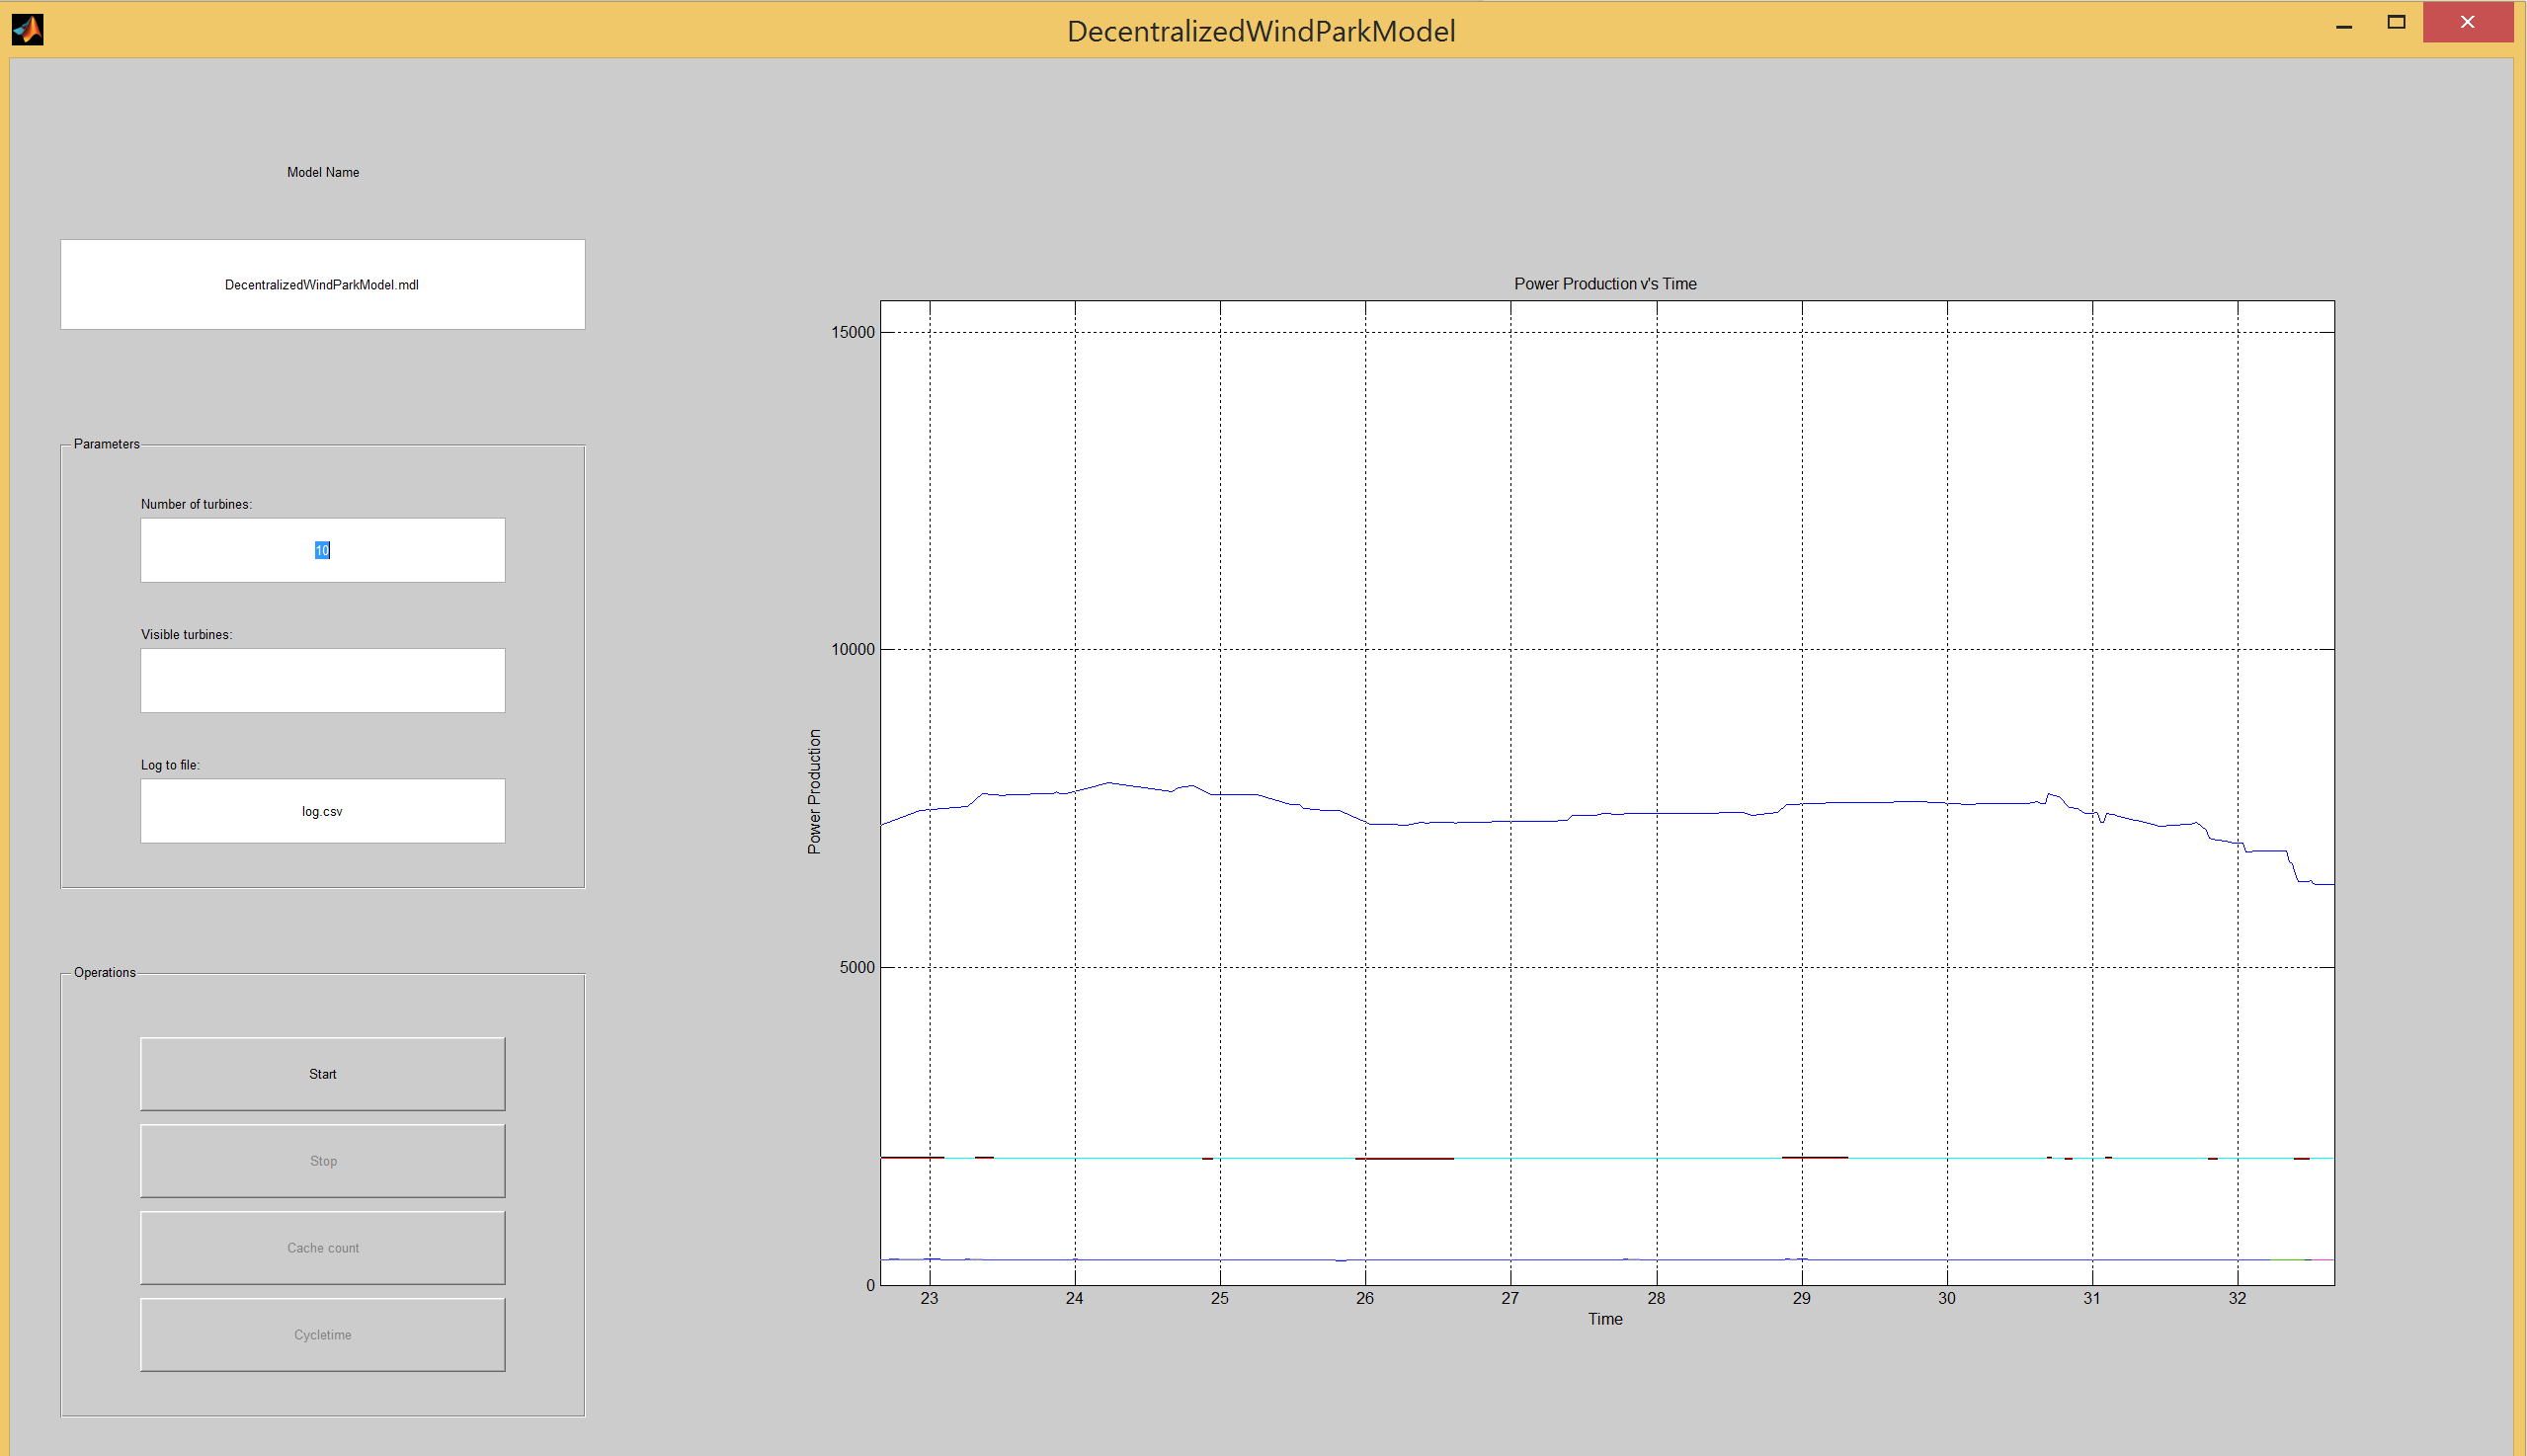
\includegraphics[width=0.9\textwidth,natwidth=610,natheight=642]{gui.png} 
	\captionsetup{format=plain,font=footnotesize,labelfont={bf,defaultCapFont},labelsep=quad,singlelinecheck=no}
	\caption[Graphical interface running 5 turbines]{
		\label{fig:graphicalInterface} 
		\footnotesize{%
			Graphical interface running 5 turbines.
		}
	}
\end{figure}


\section{\ref{PS:Q:Availability}: Remove node without system failure?}
Randomly kill client, plot a few seconds of data around the event.

\section{\ref{PS:Q:Performance}: Can we make a solution that scales?}

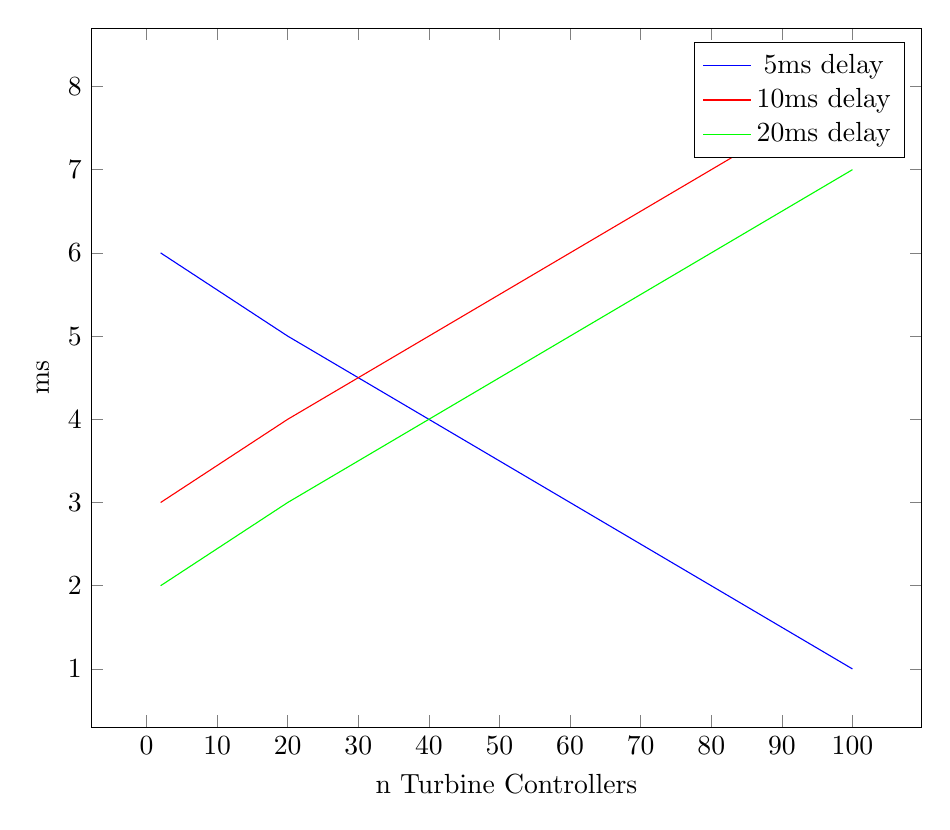
\begin{tikzpicture}
\begin{axis}[
width=\textwidth,
%ymax=0.5,
xlabel=n Turbine Controllers,
ylabel=ms]
\addplot[blue!20!blue] coordinates {
	(2 ,6)
	(20 ,5)
	(40 ,4)
	(60 ,3)
	(80 ,2)
	(100 ,1)
		};
\addplot[red!20!red] coordinates {
	(2 , 3)
	(20 ,4)
	(40 ,5)
	(60 ,6)
	(80 ,7)
	(100,8)	
	};
\addplot[green!20!green] coordinates {
		(2 , 2)
		(20 ,3)
		(40 ,4)
		(60 ,5)
		(80 ,6)
		(100,7)	
	};
\legend{5ms delay,10ms delay,20ms delay}
\end{axis}
\end{tikzpicture}



\section{\ref{PS:Q:Scalability}: Does it scale well compared to the centralized version?}
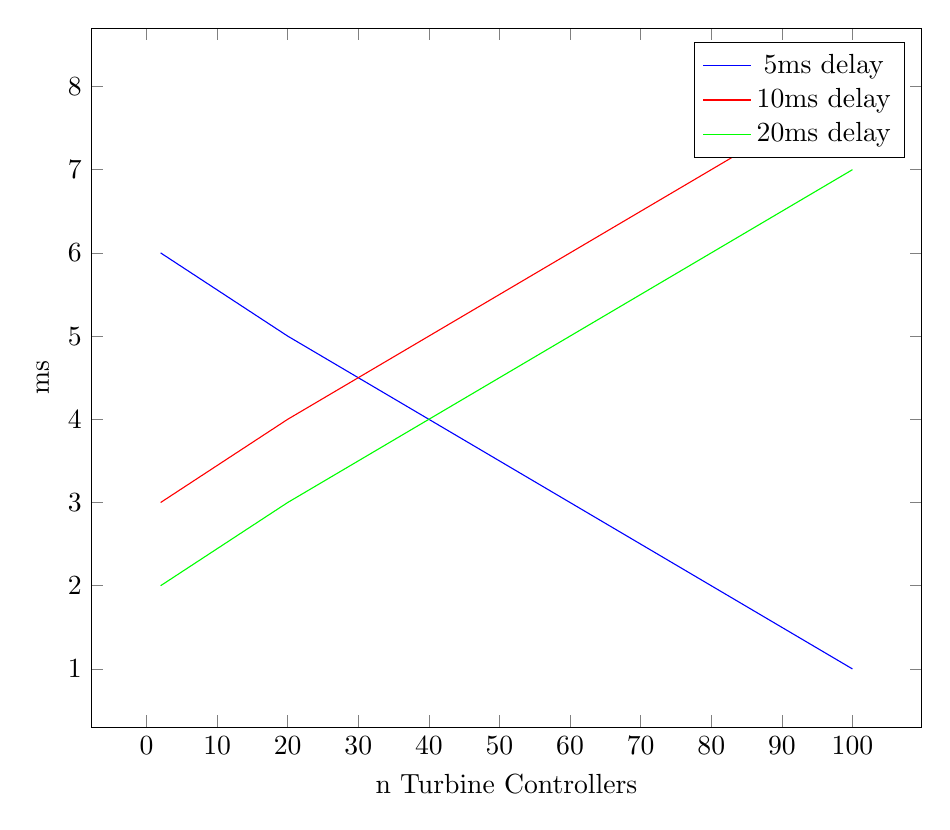
\begin{tikzpicture}
\begin{axis}[
width=\textwidth,
%ymax=0.5,
xlabel=n Turbine Controllers,
ylabel=ms]
\addplot[blue!20!blue] coordinates {
	(2 ,6)
	(20 ,5)
	(40 ,4)
	(60 ,3)
	(80 ,2)
	(100 ,1)
		};
\addplot[red!20!red] coordinates {
	(2 , 3)
	(20 ,4)
	(40 ,5)
	(60 ,6)
	(80 ,7)
	(100,8)	
	};
\addplot[green!20!green] coordinates {
		(2 , 2)
		(20 ,3)
		(40 ,4)
		(60 ,5)
		(80 ,6)
		(100,7)	
	};
\legend{5ms delay,10ms delay,20ms delay}
\end{axis}
\end{tikzpicture}


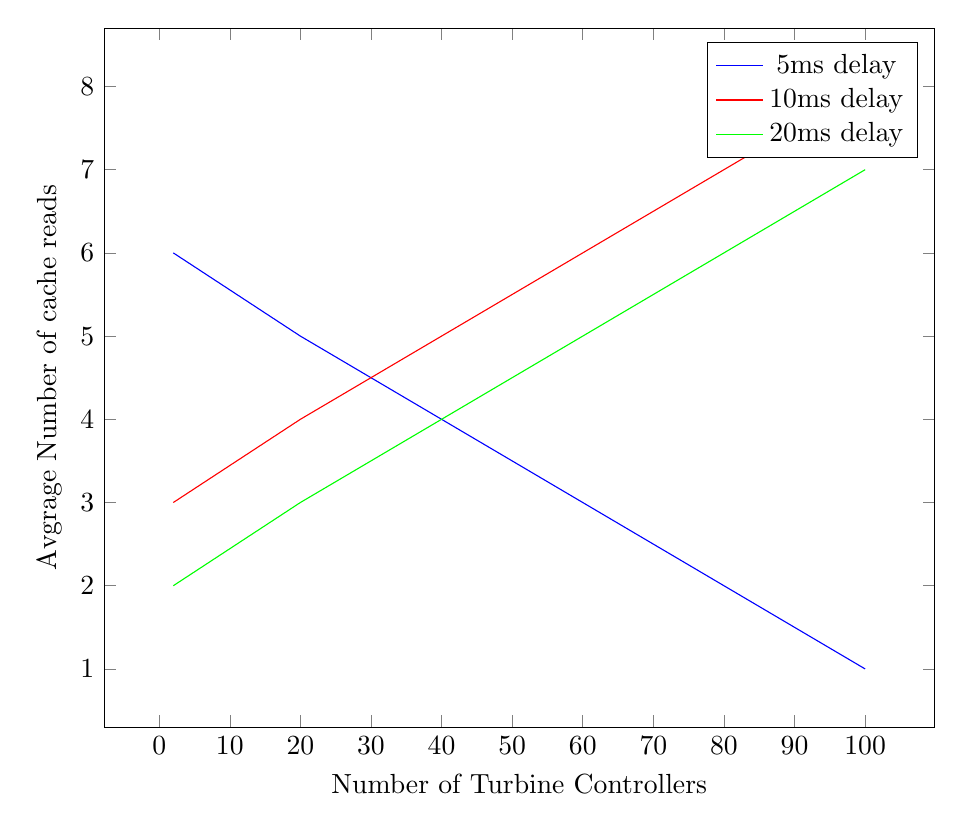
\begin{tikzpicture}
\begin{axis}[
width=\textwidth,
%ymax=0.5,
xlabel=Number of Turbine Controllers,
ylabel=Avgrage Number of cache reads]
\addplot[blue!20!blue] coordinates {
		(2 ,6)
		(20 ,5)
		(40 ,4)
		(60 ,3)
		(80 ,2)
		(100 ,1)
	};
\addplot[red!20!red] coordinates {
		(2 , 3)
		(20 ,4)
		(40 ,5)
		(60 ,6)
		(80 ,7)
		(100,8)	
	};
\addplot[green!20!green] coordinates {
		(2 , 2)
		(20 ,3)
		(40 ,4)
		(60 ,5)
		(80 ,6)
		(100,7)	
	};
\legend{5ms delay,10ms delay,20ms delay}
\end{axis}
\end{tikzpicture}

